%!TEX root = ../main.tex

This chapter describes the setup of the case study.
The \cref{fig:casestudy-workflow} depicts the overall workflow of this thesis.
In the following sections each step is elucidated.
Strong emphasis is laid on numbers and decisions.

\begin{figure}[ht]
  \centering
  \smartdiagramset{back arrow disabled=true,
    text width=.6\textwidth,
    uniform color list=black!40 for 5 items}
  \smartdiagram[flow diagram:vertical]{
    {Determine companies, keywords and stock symbols to analyze},
    {Gather data},
    {Normalization of tweets},
    {Determine sentiment of tweets},
    {Comparing sentiment time series with share prices}
  }

  \caption{Workflow of this thesis}
  \label{fig:casestudy-workflow}
\end{figure}

\section{Determine Companies, Keywords and Stock Symbols to Analyze}
\label{s:casestudy-companieskeywords}

First, a list of automotive companies is needed.
These companies must be traded on a stock exchange to perform the comparison with tweet sentiments.
As a single company may own several car brands a list of all brands has been set up.
The result of the analysis is depicted in \cref{tab:casestudy-brands}.
Both brands which aren't customer facing passenger car brands and brands which do not longer exist have been omitted.
Furthermore, the brands have been grouped by their owning company.

  \begin{longtable}[c]{!l ^l}
    \hline
    \rowstyle{\bfseries}
    Car brand & Owning Company  \\ \hline
  \endfirsthead
  %
  \multicolumn{2}{c}%
  {{\bfseries Table \thetable\ continued from previous page}} \\
   &  \\
  \endhead
  %
  BMW  & BMW \cite[p.30]{BMWGroup2017} \\
  Mini  & BMW  \cite[p.30]{BMWGroup2017} \\
  Rolls-Royce   & BMW \cite[p.30]{BMWGroup2017} \\
  Mercedes-AMG & Daimler \cite[p.90]{DaimlerAG2018} \\
  Mercedes-Benz  & Daimler \cite[p.90]{DaimlerAG2018} \\
  Mercedes-Maybach & Daimler \cite[p.90]{DaimlerAG2018} \\
  Smart  & Daimler \cite[p.90]{DaimlerAG2018} \\
  Alfa Romeo & Fiat Chrysler Automobiles \cite[p.32]{FiatChryslerAutomobiles2018a} \\
  Chrysler & Fiat Chrysler Automobiles \cite[p.32]{FiatChryslerAutomobiles2018a} \\
  Dodge & Fiat Chrysler Automobiles \cite[p.32]{FiatChryslerAutomobiles2018a} \\
  Fiat & Fiat Chrysler Automobiles \cite[p.32]{FiatChryslerAutomobiles2018a} \\
  Fiat Professional & Fiat Chrysler Automobiles \cite[p.32]{FiatChryslerAutomobiles2018a} \\
  Jeep & Fiat Chrysler Automobiles \cite[p.32]{FiatChryslerAutomobiles2018a} \\
  Lancia & Fiat Chrysler Automobiles \cite[p.32]{FiatChryslerAutomobiles2018a} \\
  RAM & Fiat Chrysler Automobiles \cite[p.32]{FiatChryslerAutomobiles2018a} \\
  Ford & Ford Motor Company \cite[p.18]{FordMotorCompany2018} \\
  Lincoln  & Ford Motor Company \cite[p.18]{FordMotorCompany2018} \\
  Baojun & General Motors Company \cite[p.1]{GeneralMotorsCompany2018} \\
  Buick & General Motors Company \cite[p.1]{GeneralMotorsCompany2018} \\
  Cadillac & General Motors Company \cite[p.1]{GeneralMotorsCompany2018} \\
  Chevrolet & General Motors Company \cite[p.1]{GeneralMotorsCompany2018} \\
  GMC & General Motors Company \cite[p.1]{GeneralMotorsCompany2018} \\
  Holden & General Motors Company \cite[p.1]{GeneralMotorsCompany2018} \\
  Jiefang & General Motors Company \cite[p.1]{GeneralMotorsCompany2018} \\
  Wuling & General Motors Company \cite[p.1]{GeneralMotorsCompany2018} \\
  Honda & Honda \cite[p.3]{HondaMotorCo.2017} \\
  Hyundai & Hyundai Motor Company \cite[p.127]{HyundaiMotorCompany2016} \\
  KIA & Hyundai Motor Company \cite[p.127]{HyundaiMotorCompany2016} \\
  Datsun & Nissan Motor Corporation \cite[p.5]{NissanMotorCorporation2017} \\
  Infinity & Nissan Motor Corporation \cite[p.5]{NissanMotorCorporation2017} \\
  Nissan & Nissan Motor Corporation \cite[p.5]{NissanMotorCorporation2017} \\
  Citroën & Groupe PSA \cite[p.3]{GroupePSA2018} \\
  Opel & Groupe PSA \cite[p.3]{GroupePSA2018} \\
  Peugeot& Groupe PSA \cite[p.3]{GroupePSA2018} \\
  Vauxhall & Groupe PSA \cite[p.3]{GroupePSA2018} \\
  Alpine & Groupe Renault \cite[p.11]{GroupeRenault2018} \\
  Dacia & Groupe Renault \cite[p.11]{GroupeRenault2018} \\
  Lada & Groupe Renault \cite[p.11]{GroupeRenault2018} \\
  Renault & Groupe Renault \cite[p.10]{GroupeRenault2018} \\
  Renault Samsung Motors & Groupe Renault \cite[p.10]{GroupeRenault2018} \\
  Daihatsu & Toyota Motor Corporation \cite[p.2]{ToyotaMotorCorporation2018} \\
  Lexus & Toyota Motor Corporation \cite[p.2]{ToyotaMotorCorporation2018} \\
  Toyota & Toyota Motor Corporation \cite[p.2]{ToyotaMotorCorporation2018} \\
  Audi & Volkswagen AG \cite[p.104]{VolkswagenAktiengesellschaft2017} \\
  Bentley & Volkswagen AG \cite[p.104]{VolkswagenAktiengesellschaft2017} \\
  Bugatti & Volkswagen AG \cite[p.104]{VolkswagenAktiengesellschaft2017} \\
  Lamborghini & Volkswagen AG \cite[p.104]{VolkswagenAktiengesellschaft2017} \\
  Porsche & Volkswagen AG \cite[p.104]{VolkswagenAktiengesellschaft2017} \\
  Seat & Volkswagen AG \cite[p.104]{VolkswagenAktiengesellschaft2017} \\
  Škoda & Volkswagen AG \cite[p.104]{VolkswagenAktiengesellschaft2017} \\
  Volkswagen & Volkswagen AG \cite[p.104]{VolkswagenAktiengesellschaft2017} \\ \hline
  
  \caption{Automotive brands and their corresponding owning company}
  \label{tab:casestudy-brands}
  \end{longtable}

According to the survey of \emph{World Motor Vehicle Production 2016} the biggest five car manufacturing companies are: Toyota, Volkswagen, Hyundai, General Motors and Ford \cite{OICA2016}.
Therefore the study will focus on these five companies.
The count of manufactured cars and the companies stock symbol are summarized in \cref{tab:casestudy-companies-counts-and-symbols}.
The containing symbols in the table are derived by literature research and using the Yahoo Finance portal (\url{https://finance.yahoo.com}).

\begin{table}
  \begin{tabular}[c]{!l ^r ^l ^l}
    \hline
    \rowstyle{\bfseries}
	  Company & \#cars \cite{OICA2016} & Stock Exchange & Symbol  \\ \hline
	  Ford Motor Company & 6,429,485 & New York \cite{FordMotorCompany2018} & F  \\
	  General Motors Company & 7,793,066 & New York \cite[p.17]{GeneralMotorsCompany2018} & GM \\
	  Hyundai Motor Company & 7,889,538 & Korea \cite[p.92]{HyundaiMotorCompany2016} & 005380.KS \\
	  Toyota Motor Corporation & 10,213,486 & Tokyo \cite{ToyotaMotorCorporation2018} & 7203.T \\
	  Volkswagen AG & 10,126,281 & Frankfurt \cite[p.110]{VolkswagenAktiengesellschaft2017} & VOW.F \\  \hline
	\end{tabular}
	\caption{Automotive companies and their corresponding produced cars and stock symbol}
	\label{tab:casestudy-companies-counts-and-symbols}
\end{table}

\section{Gather Data}
\label{s:casestudy-gatherdata}

Gathering data is split into two different tasks:
gathering tweets which is described in detail in \cref{ss:casestudy-gatherdata-tweets}, 
and gather stock prices which is described in \cref{ss:casestudy-gatherdata-stockprices}.

\subsection{Gather Tweets}
\label{ss:casestudy-gatherdata-tweets}

A large set of tweets is needed to perform the analysis within a time frame of at least one month.
There were several approaches to get these tweets: download tweets directly or capture tweets within the given time frame.
As we are tracking five companies using 23 keywords (brands) there will be a quite big amount of data.

Several approaches have been tried to get as many tweets as possible to the given keywords, including:

\begin{description}
  \item [Official Twitter search \ac{API}] 
    was the first attempt.
    But there were very serious limitations to the official \ac{API} that made that quite easy way impossible.
    First, the standard search \ac{API} supports just a maximum count of 100 tweets;
    second, it supports a history of only seven days;
    and lastly, there were to tight rate limits defined in order gather all possible tweets of the seven days period \cite{TwitterInc.2018}.

  \item [Twitter search on website]
    has been tried to overcome the shortcomings of the official Twitter \ac{API} but the tweets cannot be downloaded in a easy way as the results only appear within the web browser.
    A Java tool (\url{https://github.com/Jefferson-Henrique/GetOldTweets-java}) has been found which tries to exploit the search page and extract tweets from the website.
    But this tool did not work as expected.
    Most likely Twitter made some changes to the search result page and the tool has not been adopted since \printdate{2016-04-15} \cite{Jefferson2016}.

  \item [DMI TCAT]
    is a toolset for capturing and analyzing tweets.
    It has been developed by \citeauthor{Borra2014} to support researchers around the globe and make tweet collection and analysis easier
    \cite{Borra2014}.
    TCAT support various ways of data capturing:
    \begin{itemize}
      \item One percent random sample of all tweets passing through Twitter,
      \item Streaming endpoint of the \ac{API} to track up to 400 keywords,
      \item Following up to 5000 specified users, such as members of a parliament or other expert lists \cite{Borra2014}.
    \end{itemize}

\end{description}

After exploring all of these methods DMI TCAT has been selected to capture the necessary Twitter data by using the streaming endpoint of the \ac{API} to track 23 keywords.
The tool must be installed on a computer in order to perform its work.
As the tool need some serious amount of capacities and need to collect tweets 24/7 it has been installed on a virtual machine in the Microsoft Azure cloud.

The 23 keywords have been grouped by the owning company into so called query bins.
A query bin may contain multiple keywords to track and combine all identified tweets into one single data set \cite{Borra2014}.

All tweets have been captured between \printdate{2018-02-28} to \printdate{2018-09-06}.
But there were several issues using the cloud approach:

\begin{itemize}

  \item By default the virtual machine in the cloud shut down every day on 7 PM.
    First a problem with the tool was expected but after several days and starting the virtual machine manually the origin of the issue was discovered and solved.

  \item The storage space of the virtual machine initialized with 30 \ac{GB}, which was too small for the collected tweet amount.
    The storage was full after approximately 14 days of data collection.
    As the problem was not detected right away it took several days for identifying and fixing the issue.

  \item The rate limits of the \ac{API} have been hit now and then in case too many tweets were published.
    DMI TCAT continued to collect tweets automatically after the corresponding time window.

  \item New releases DMI TCAT have been published from time to time which also required a database upgrade.
    As the performance was dropping the upgrade was performed in the hope of fixing the performance issue.
    Furthermore, the first update was needed to enable DMI TCAT to process tweets longer than 140 characters.
    The database upgrade needed to suspend the tweet collection by a serious amount of time.
    To collect as many tweets as possible the upgrade was performed in steps for each query bin separately.
    The larger the query bin the longer the process took as every single tweet was needed to be altered.

\end{itemize}

The number of collected tweets can be seen in \cref{tab:casestudy-companies-numberoftweets}.

\begin{table}[hbt]
  \centering
  \begin{tabular}{!l ^r ^r}
    \hline
    \rowstyle{\bfseries}
  Company & \# captured tweets & \# english tweets  \\ \hline
    Ford & \num{4518198} & \num{3745490} \\
    General Motors & \num{575547} & \num{413817} \\
    Hyundai & \num{1895306} & \num{697277} \\
    Toyota & \num{915868} & \num{488913} \\
    Volkswagen & \num{8244083} & \num{6219786} \\ \hline
    Total & \num{16149002} & \num{11565283} \\ \hline
  \end{tabular}

  \caption{Numbers of collected tweets}
  \label{tab:casestudy-companies-numberoftweets}
\end{table}

\subsection{Gather Stock Prices}
\label{ss:casestudy-gatherdata-stockprices}

The stock data can be downloaded at any point of time for the given research period on a daily frequency basis using the Yahoo Finance website.
The stock prices in a time frame of a year have been downloaded which contains the period of tweet collection.

The data contains the following information for each day:
Date, Open, High, Low, Close, Adj. Close and Volume.

% \begin{description}
%   \item [Date] on which the data applies
%   \item [Open]
% \end{description}

\section{Normalization of Tweets}
\label{s:casestudy-normalization}

Prior analysis the tweets have been preprocessed which is also called normalization.
The importance of normalization has been described in \cref{ss:background-optionmining-textfeatureextraction}.

In the following the steps of normalization are described in detail:

\begin{description}

  \item [Lower case:]
    The tweet text is converted to lower case as the meaning stays the same but the dictionary size is reduced.

  \item [Tokenization:]
    For tokenization the \emph{TweetTokenizer} of the NLTK package is used.
    This tokenizer has been created for this purpose.

  \item [Stopwords:]
    The predefined english stopwords of the NLTK package have been removed from all tweets.
  
  \item [Lemmatization:]
    There are several lemmatizer available and the \emph{WordNetLemmatizer} of the NLTK package is used to perform this step.

  \item [Stemming:]
    The same situation applies to stemmers.
    The \emph{SnowballStemmer} of the NLTK package is used as many found examples used this specific stemmer.

  \item [Custom \ac{RegEx}:]
    Last but not least, custom \ac{RegEx} have been used to remove or replace other unwanted elements of tweets, such as \cite{Pagolu2016a}:

    \begin{enumerate}
      \item User references (``@someuser'') are replaced with the generic word ``user''.
      \item Specific URI are replaced with the word ``uri''.
      \item Three or more consecutive characters are replaced by two consecutive characters.
        For example: the word ``coooooooool'' becomes ``cool''.
      %\item Questionmarks are replaced by the word ``question'' and exclamationmarks are replace by the word ``exclamation''.
      \item Hashtags have been removed as the hash symbol does not provide any additional information. 
        For example: the hashtag ``\#cool'' is replaced by ``cool''.
    \end{enumerate}

\end{description}

As these described normalization steps are language sensitive only english tweets are used for this and following steps.

\section{Determine Sentiment of Tweets}
\label{s:casestudy-sentiment}
% maybe useful?
% https://github.com/ayushoriginal/Sentiment-Analysis-Twitter

After normalization the tweets were ready for sentiment detection.
The sentiments were detected using four different classifiers using the same workflow depicted in \cref{fig:casestudy-sentimentworkflow}, the used symbols are described in \cref{tab:casestudy-sentimentvariables} and the same pipeline configuration depicted in \cref{fig:casestudy-sentimentpipeline}.

\begin{table}[hbt]
  \centering
  \begin{tabular}{!l ^l}
    \hline
    \rowstyle{\bfseries}
    Symbol & Description \\ \hline
    $T_S$ & Sample tweets \\
    $T_C$ & Collected tweets \\
    $P$   & Pipeline \\
    $P_T$ & Trained pipeline \\
    $S$   & Sentiment \\ \hline
  \end{tabular}

  \caption{Variable definitions for sentiment detection}
  \label{tab:casestudy-sentimentvariables}
\end{table}

\begin{figure}[hbt]
  \centering
  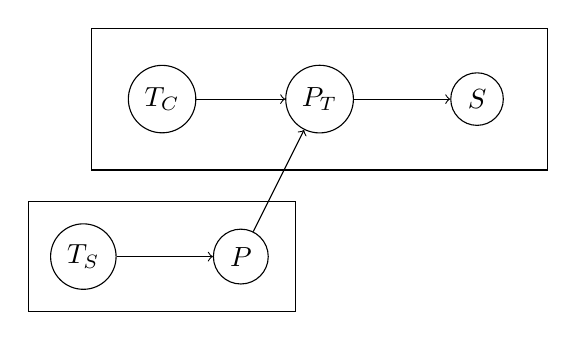
\begin{tikzpicture}
    \node (ts) at (0,0) [circle, draw] {$T_S$};
    \node (p) at (2,0) [circle, draw] {$P$};
    \node (tc) at (1,2) [circle, draw] {$T_C$};
    \node (pt) at (3,2) [circle, draw] {$P_T$};
    \node (s) at (5,2) [circle, draw] {$S$};

    \draw[->] (ts) -- (p);
    \draw[->] (tc) -- (pt);
    \draw[->] (p) -- (pt);
    \draw[->] (pt) -- (s);

    \draw (-.7,-.7) rectangle (2.7,.7);
    \draw (0.1,1.1) rectangle (5.9,2.9);
  \end{tikzpicture}

  \caption{Workflow for sentiment detection}
  \label{fig:casestudy-sentimentworkflow}
\end{figure}

\begin{figure}[hbt]
  \centering
  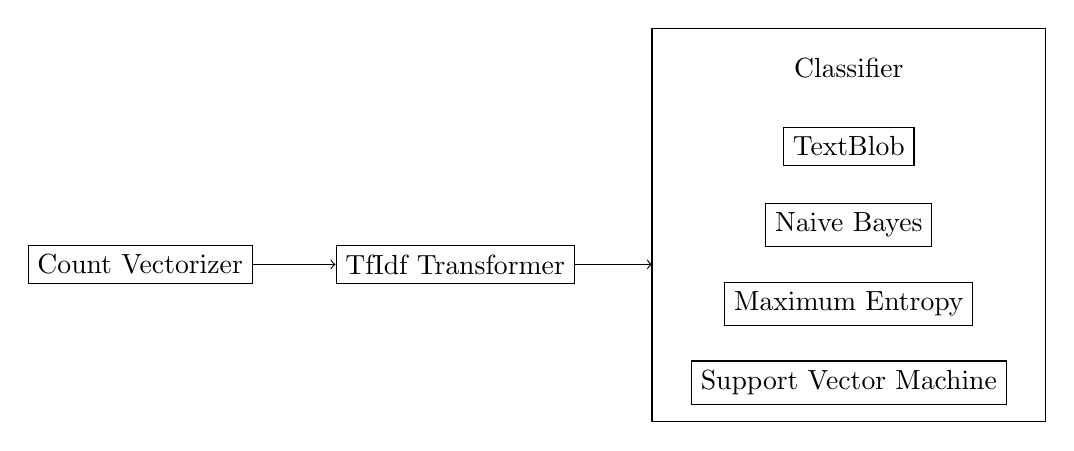
\begin{tikzpicture}
    \node (cv)     at (0,0) [rectangle, draw] {Count Vectorizer};
    \node (tfidf)  at (4,0) [rectangle, draw] {TfIdf Transformer};

    \node (cf_tb)  at (9,1.5) [rectangle, draw] {TextBlob};
    \node (cf_nb)  at (9,0.5) [rectangle, draw] {Naive Bayes};
    \node (cf_me)  at (9,-0.5) [rectangle, draw] {Maximum Entropy};
    \node (cf_svm) at (9,-1.5) [rectangle, draw] {Support Vector Machine};

    \node (cf)     at (9,2.5) {Classifier};
    
    \draw (6.5,-2) rectangle (11.5,3);

    \draw[->] (cv) -- (tfidf);
    \draw[->] (tfidf) -- (6.5,0);
  \end{tikzpicture}

  \caption{Pipeline for sentiment detection}
  \label{fig:casestudy-sentimentpipeline}
\end{figure}

%buitinck2013api

Pipelines are a useful construct provided by the \emph{scikit-learn} project.
The basic philosophy in this project is to divide the public \ac{API} into four parts:

\begin{description}
  \item [Data representation.]
    In most machine learning tasks the data is modeled as a set of variables.
    In supervised learning tasks the goal is to find a mapping from various input variables to some output variables.
    A common way to represent such a dataset is a pair of matrices: one for the input values and one for the output values.
    Within one matrix one column corresponds to one variable and one row corresponds to a specific sample of the problem.
    To construct such matrices from textual data \emph{scikit-learn} provides \emph{vectorizer} objects
    \cite{buitinck2013api}.

  \item [Estimators.]
    Machine learning tasks are designed as \emph{estimator} objects which expose a \emph{fit} method.
    It provides the separation of model creation and learning.
    A model is initialized with specific parameters regarding the specific task which are also called \emph{hyper-parameters}.
    The actual learning is provided by the \emph{fit} method which takes two matrices as input parameters at least for supervised learning algorithms.
    After fitting the parameters to the training data the model is trained and can be used to perform predictions or transformations
    \cite{buitinck2013api}.

  \item [Predictors.]
    \emph{Predictors} are used to produce target variables by a given set of input variables.
    The \emph{predict} method is also supplied by the same model object which has been trained before by using the \emph{fit} method.
    Beside the \emph{predict} method predictors have to provide a \emph{score} method which quantifies the quality of the predictions.
    For supervised learning models the \emph{score} method takes two matrices as input parameters: input data and expected output data.
    Using the import data the model then predicts the output values and calculates the difference to the expected output values.
    The higher the calculated score is the better is the quality of the prediction
    \cite{buitinck2013api}.

  \item [Transformers.]
    Usually data is modified or filtered before it is used for model training or prediction.
    Therefore \emph{scikit-learn} provides objects with the \emph{transformer} interface which exposes a method called \emph{transform}.
    The method takes an input parameter for input values and generates a transformed matrix of input values.
    \emph{Transformers} can be used to scale values to the standard normal distribution
    \cite{buitinck2013api}.

\end{description}

\emph{Scikit-learn} provides furthermore a mechanism to combine several estimators to a new estimator which than can be used such as a basic estimator.
To provide a simple sequential workflow of feature extraction, transforming, fitting and prediction \emph{scikit-learn} provides pipeline objects.
The pipeline is a useful construct to perform the same steps over and over in a standardized way for training and estimation
\cite{buitinck2013api}.

% Cross validation with GridSearchCV
Furthermore \emph{scikit-learn} provides some helpers to find the best hyper-parameters for the given problem.
The user can define which values various hyper-parameters can attain and the helper then perform test runs for various combinations, calculate their score and keep acting as the best performing model.
Therefore, this type of search is called \emph{model selection}.
\emph{Scikit-learn} provides two different model selection helpers: \emph{GridSearchCV} and \emph{RandomizedSearchCV}.
Whereas \emph{GridSearchCV} generates a \emph{grid} of the complete combinatorial combinations and perform the scoring with every single combination, \emph{RandomizedSearchCV} takes a fixed number of parameter combinations
\cite{buitinck2013api}.

The model selection helper of \emph{scikit-learn} can also perform a cross-validation.
By default \emph{GridSearchCV} uses \emph{k-fold} cross-validation by optimizing the \emph{score} function of the estimator.
The value which should be optimized can be changed to a variety of predefined key figures including the $F-Measure$
\cite{buitinck2013api}.

In this thesis the \emph{GridSearchCV} model selection helper is used. 
In the following sections each part of the pipeline and tried hyper-parameters used are described.

\begin{description}
  \item[Count Vectorizer] 
    The count vectorizer is used to generate both a vocabulary and a numerical representation of the normalized tweets.
        
    \begin{table}[!hbt]
      \centering
      \begin{tabular}{!l ^l}
        \hline
        \rowstyle{\bfseries}
        Variable & Tried values \\ \hline
        NGrams & 1-gram to 4-grams \\
        Stopwords & none \\
        Binary & true, false \\ \hline
      \end{tabular}
    
      \caption{Hyper-parameters of the CountVectorizer}
      \label{tab:casestudy-hyperparams-countvectorizer}
    \end{table}
  

  \item[\ac{TF-IDF} Transformer]
    The \ac{TF-IDF} is used to transform the vocabulary from the count vectorizer to make common words less important for the analysis.
    The implementation used also supports to deactivate the transformation at all.
    If the untransformed vocabulary would lead to better results the GridSearchCV would figure that out and use the best set of parameters.
    All hyper-parameters for the transformer can be found in \cref{tab:casestudy-hyperparams-tfidftransfomer}.
  
    \begin{table}[!hbt]
      \centering
      \begin{tabular}{!l ^l}
        \hline
        \rowstyle{\bfseries}
        Variable & Tried values \\ \hline
        Use IDF & true, false \\
        Smooth IDF & true \\
        Normalization & 'l1', 'l2', none \\ \hline
      \end{tabular}
    
      \caption{Hyper-parameters of the \ac{TF-IDF} Transformer}
      \label{tab:casestudy-hyperparams-tfidftransfomer}
    \end{table}
  
    
  \item[Classifier]
    The pipeline has been tried using four different classifiers.
    Each of them has different hyper-parameter.
    Therefore, they will be discussed in the corresponding sections.

    \begin{description}
      \item[TextBlob Classifier]
      
        The TextBlob classifier is a pre-trained classifier which has no hyper-parameters at all.
        It works out of the box.
        The only effort made was to make the TextBlob classifier available to the scikit-learn package by implementing the estimator interface (the method \emph{predict}).
        
      \item[Naive Bayes Classifier]
        The Naive Bayes classifier was the first classifier which supported hyper-parameters.
        As the philosophy of \emph{scikit-learn} is to provide good default values only some hyper-parameters have been modified
        \cite{buitinck2013api}.
        The implementation used is class \emph{sklearn.naive\_bayes.MultinomialNB}.
        All tried hyper-parameter values are depicted in \cref{tab:casestudy-hyperparams-nbclassifier}.
      
        \begin{table}[!hbt]
          \centering
          \begin{tabular}{!l ^l}
            \hline
            \rowstyle{\bfseries}
            Variable & Tried values \\ \hline
            Alpha & $10^{-2}$, $10^{-3}$ \\ \hline
          \end{tabular}
        
          \caption{Hyper-parameters of the Naive Bayes Classifier}
          \label{tab:casestudy-hyperparams-nbclassifier}
        \end{table}
        
      \item[Maximum Entropy Classifier]
        The implementation used for the Maximum Entropy classifier is class \emph{sklearn.linear\_model.LogisticRegression} which have some built in solvers.
        The tried solvers and other hyper-parameters can be found in \cref{tab:casestudy-hyperparams-meclassifier}.
      
        \begin{table}[!hbt]
          \centering
          \begin{tabular}{!l ^l}
            \hline
            \rowstyle{\bfseries}
            Variable & Tried values \\ \hline
            Solver & 'liblinear', 'lbfgs', 'sag', 'saga' \\
            Multiclass & 'auto' \\ \hline
          \end{tabular}
        
          \caption{Hyper-parameters of the Maximum Entropy Classifier}
          \label{tab:casestudy-hyperparams-meclassifier}
        \end{table}
        
      \item[Support Vector Machine Classifier]
        The Support Vector Machine classifier used is class \emph{sklearn.linear\_model.SGDClassifier} with loss function 'hinge' as this is the only support loss function which results in a linear \ac{SVM}.
        Other hyper-parameters can be found in \cref{tab:casestudy-hyperparams-svmclassifier}.
      
        \begin{table}[!hbt]
          \centering
          \begin{tabular}{!l ^l}
            \hline
            \rowstyle{\bfseries}
            Variable & Tried values \\ \hline
            Tolerance & $10^{-2}$, $10^{-3}$ \\
            Loss & 'hinge' \\ \hline
          \end{tabular}
        
          \caption{Hyper-parameters of the Support Vector Machine Classifier}
          \label{tab:casestudy-hyperparams-svmclassifier}
        \end{table}
        
    \end{description}

    A pipeline is built for each classifier.
    The GridSearchCV model selector is used to train the specific pipeline using the hyper-parameters defined to find the best possible parameters for each component.

    The sentiment analysis is then performed with the selected model and stored in files for further analysis.

  \item[Comparing Sentiment Time Series with Share Prices]
    
    Both datasets, stock prices and sentiment analysis results respectively, are stored in files prior the comparison.
    The stock prices are already in a time series format on a daily basis except for weekends or holidays but the problem of missing entries are tackled later.
    First, the sentiment analysis result dataset must be condensed to form a time series for comparison.
    Therefore the results per tweet are grouped per day and summed up.
    As negative sentiments have the value \texttt{'-1'} and positive sentiments have the value \texttt{'1'} we receive a number which is positive in case more positive than negative tweets have been published on that given day and vice versa. 

    Missing stock prices have been calculated iteratively and the gaps have been filled by using the following procedure:
    Given $x$ is a stock price value and $y$ is the next present value with one or more values in between are missing.
    The missing values are calculated using the formula $\frac{x+y}{2}$.
    The formula is applied to the first missing value then the calculated value is treated as new $x$ and so on.
    These steps are repeated as long values were missing
    \cite{Pagolu2016a}.    
    To fill the gaps of sentiment time series the same iterative approach as for stock prices has been chosen.

    Afterwards, the time series have been analyzed using Granger causality analysis.

\end{description}